\documentclass{mistcoursedoc}
\usepackage[french]{babel}
\usepackage[utf8]{inputenc}
\usepackage{paralist}


\course{INF3995: Projet de conception d’un\\ système informatique}
\term{Hiver}
\termyears{2021} 
\doctype{Réponse à l’appel d’offres}

% Numéro équipe
\newcommand{\equipe}{203}

\author{Équipe \equipe}

\begin{document}

\maketitle
\vspace{2cm}
\begin{center}

  {\Huge\bf Système aérien minimal pour exploration\\[3em]}

  \Large Proposition répondant à l’appel d’offres  n°H2021-INF3995 du département GIGL\\[3em]


  Équipe No. \equipe\\[3em]

  Bal, Samba Bousso\\[1em]
  Chritin, Mathurin\\[1em]
  Grootenboer, Hubert\\[1em]
  Maghni, Issam Eddine\\[1em]
  Sangam, Eya-Tom Augustin\\[1em]

  \vfill

\end{center}

\newpage
{
    \renewcommand{\contentsname}{Table des matières}
    \hypersetup{hidelinks}
    \setcounter{secnumdepth}{3}
    \setcounter{tocdepth}{3}
    \tableofcontents
}
\newpage

\section*{Introduction}

Bla bla bla

\section{Vue d’ensemble du projet}

\subsection{But du projet, porté et objectifs}

\textit{Décrire brièvement le but et les objectifs du projet ainsi que des biens livrables attendus.}

\par L'objectif principal de ce projet est de créer un système informatique de gestion de drones.
Le dit système permettra à son utilisateur d'explorer et cartographier un milieu arbitraire depuis une station au sol.
Le système pourra faire marcher ensemble une colonie de drones, communiquant entre eux, pour fournir une cartographie du milieu exploré.

\par Un tel système se vaudra très utile durant les explorations sur Mars, encore peu connue de tous.
Nous imaginons une situation dans laquelle, un robot plus complexe,
plus lent et limité dans sa capacité de mouvement, se fera diriger par une colonie de drones qui
lui indiquera les endroits les plus intéressants à explorer.

\subsection{Hypothèse et contraintes}

\textit{Énumérer les hypothèses sur lesquelles repose ce plan ainsi que les contraintes dans le cadre de ce projet.
Pas seulement des éléments techniques, mais aussi des éléments externes à l’équipe.}

\subsubsection{Hypothèses sur l'utilisation du système}

\begin{itemize}

  \item \textbf{Utilisation du système} :\\
  Le système conçu sera utilisé uniquement à des fins d'explorations et non d'espionnage. 
  Selon le milieu exploré,l'utilisateur du système se devra d'obtenir les autorisations nécessaires conformément au lois régissant l'utilisation
  des drones de le province concernée.

  \item \textbf{Sécurité} :\\
  L'opérateur du système devra être âgé d'au moins 16 ans et devra se munir de lunettes de sécurité durant toute
  manipulation affectant les drones.

  \item \textbf{Milieu exploré} :\\
  Le milieu exploré devra se trouver dans des conditions métrologiques convenable. 
  Idéalement, une pièce fermé à température ambiante.

  \item \textbf{Équipement de base} :\\
  L'opérateur du système devra posséder au moins deux kits Crazyfly 2.0 Stem Bundle.
  L'ordinateur de la station de contrôle devra être muni d'un système d'exploitation 
  Linux virtualisé ou non possédant au minimum 4 Giga Octets de mémoire vive. Y devront êtres installés 
  au minimum un navigateur graphique de nouvelle génération ainsi qu'un invité de commande bash.\\
  
\end{itemize}

\subsubsection{Contraintes fonctionnelles}
Le système devrait être en mésure de répondre au contraintes ci-dessous :

\begin{itemize}
  \item Une fois la commande de départ reçue, les drones doivent être capables de parcourir le périmètre 
  d’une pièce de maximum 100 m2 en absence d’autres commandes de la station au sol.
  \item Le système doit être conçu pour fonctionner idéalement avec un nombre arbitraire de drones, 
  ne tenant pas compte du système de communication avec la station au sol, mais jamais moins que deux(2).
  \item Les drones doivent éviter les obstacles sur leur chemin, incluant les autres drones.
  \item L’essaim de drones doit répondre au minimum aux commandes suivantes, disponibles sur l’interface utilisateur
\end{itemize}

\subsubsection{Contraintes de temps}
La charge requise en termes d’heures pour la livraison du projet est de 630 heures-personnes. 
Plus de détails sont disponibles plus bas. // TODO : Ajouter un lien vers la section.
Un version finale du projet sera livrée pour le lundi 12 avril 2021 en avant-midi.


\subsection{Biens livrables du projet}
\textit{Énumérer les artéfacts qui devront être créés durant le projet avec leurs dates prévues de publication.}


3 briques : dashboard, serveur maître + base de données, firmware
\begin{itemize}
  \item \textbf{Prototype minimal} : afin de démontrer au client la maîtrise des technologies utilisées (\textit{date prévue 2021-02-15}):
        \begin{itemize}
          \item Interface web minimale avec boutons « Take Off » et « Land », ainsi que le niveau de batterie, la position et la vitesse du drone en action dans le simulateur Argos 3
          \item Serveur maître basique faisant l'intermédiaire entre le simulateur et l'interface web : relais des messages de mise à jour temps réel des drones vers le client web, et transfert des commandes du client web vers les drones, le tout à l'aide d'une socket TCP. Pas encore de concept de base de donnée.
          \item Version basique du micrologiciel : récupération des données de la batterie et de la vitesse, encodage sous forme \texttt{json} et envoie des données vers une socket TCP
          \item Simulateur Argos faisant bouger deux drones
        \end{itemize}
  \item \textbf{Prototype intermédiaire} : pour démontrer au client l'avancement du projet (\textit{date prévue 20201-03-08}) :
      \begin{itemize}
        \item Interface web avancée, avec boutons « TakeOff » et « Return to base » implémentés, et visualisation minimale des données captées par le drone
        \item Simulateur avec 4 drones évoluant dans un environnement généré aléatoirement en évitant les obstacles
        \item Serveur maître et micrologiciel avancés pour répondre aux besoins de la démonstration décrite par les points ci-dessus
      \end{itemize}
      % TODO move somewhere else
      % \begin{itemize}
      %   \item Interface web évoluée, avec de quoi afficher les données visualisées par le drone en temps réel sous forme de graphe.
      %   \item Serveur maître évolué, implémentant un premier modèle de base de donnée capable de stocker en temps réel des données quelconques (en attendant de pouvoir stocker les informations sur les obstacles émises par les drones).
      %   \item Micrologiciel évolué : capable de retrouver les données des capteurs de distance et de les interpréter pour faire varier l'itinéraire du drone en fonction de ces informations.
      % \end{itemize}
  \item \textbf{Démonstration finale}, mettant en jeu :
      \begin{itemize}
        \item L'interface web finale avec les boutons « TakeOff » et « Return to base » comme seules commandes pour lancer et terminer la mission, et affichage de toutes les informations des drones en temps réel
        \item Le serveur maître final pour interfacer les commandes de l'interface web et traiter les données reçues des drones
        \item Le tout sous la forme d'une vidéo pour montrer le comportement des drones dans un environnement qu'il ne connaît pas
      \end{itemize}
\end{itemize}

\section{Organisation du projet}

\subsection{Structure d’organisation}

\textit{Décrire la structure d’organisation de l’équipe de projet et les différents rôles des membres.}
L'équipe est composée de 5 membres. Les 5 membres participeront au développement de la solution à tous les niveaux (client, serveur et micrologiciel), et seront en tout temps au courant de l'avancement des différents artéfacts du projet. Un membre de l'équipe, M. Samba Bal, assumera le rôle du gestionnaire de projet pour organiser le développement. GitLab sera utilisé pour gérer les tâches à effectuer, les assigner aux différents membres et comptabiliser le temps passé sur chacune d'elles.

\subsection{Entente contractuelle}

\textit{Décrire le type d’entente contractuelle proposée pour projet et les raisons de ce choix}

Un contrat de livraison clef en main serait adéquat pour ce projet. En effet, le contracteur a une liste des requis complete et suffisamment précise pour ne pas avoir a la modifier grandement au cours du projet.
Grace à cela, on peut prévoir le temps qu'il faudra pour réaliser le projet et ainsi prévoir un coup fixe pour la réalisation du produit.

\section{Solution proposée}

\subsection{Architecture logicielle générale}

\textit{Un diagramme qui résume l’architecture.  Un texte qui décrit et justifie les choix. Inspiration: \og L’ingénieur a parfois un peu peur de réaliser des choses parce que les moyens sont maintenant considérablement sophistiqués. On oublie que seulement prendre un papier et un crayon, décrire les choses, faire une esquisse, cela peut être aussi valable qu’un dessin d’ordinateur.}

\begin{figure}[h!]
  \centering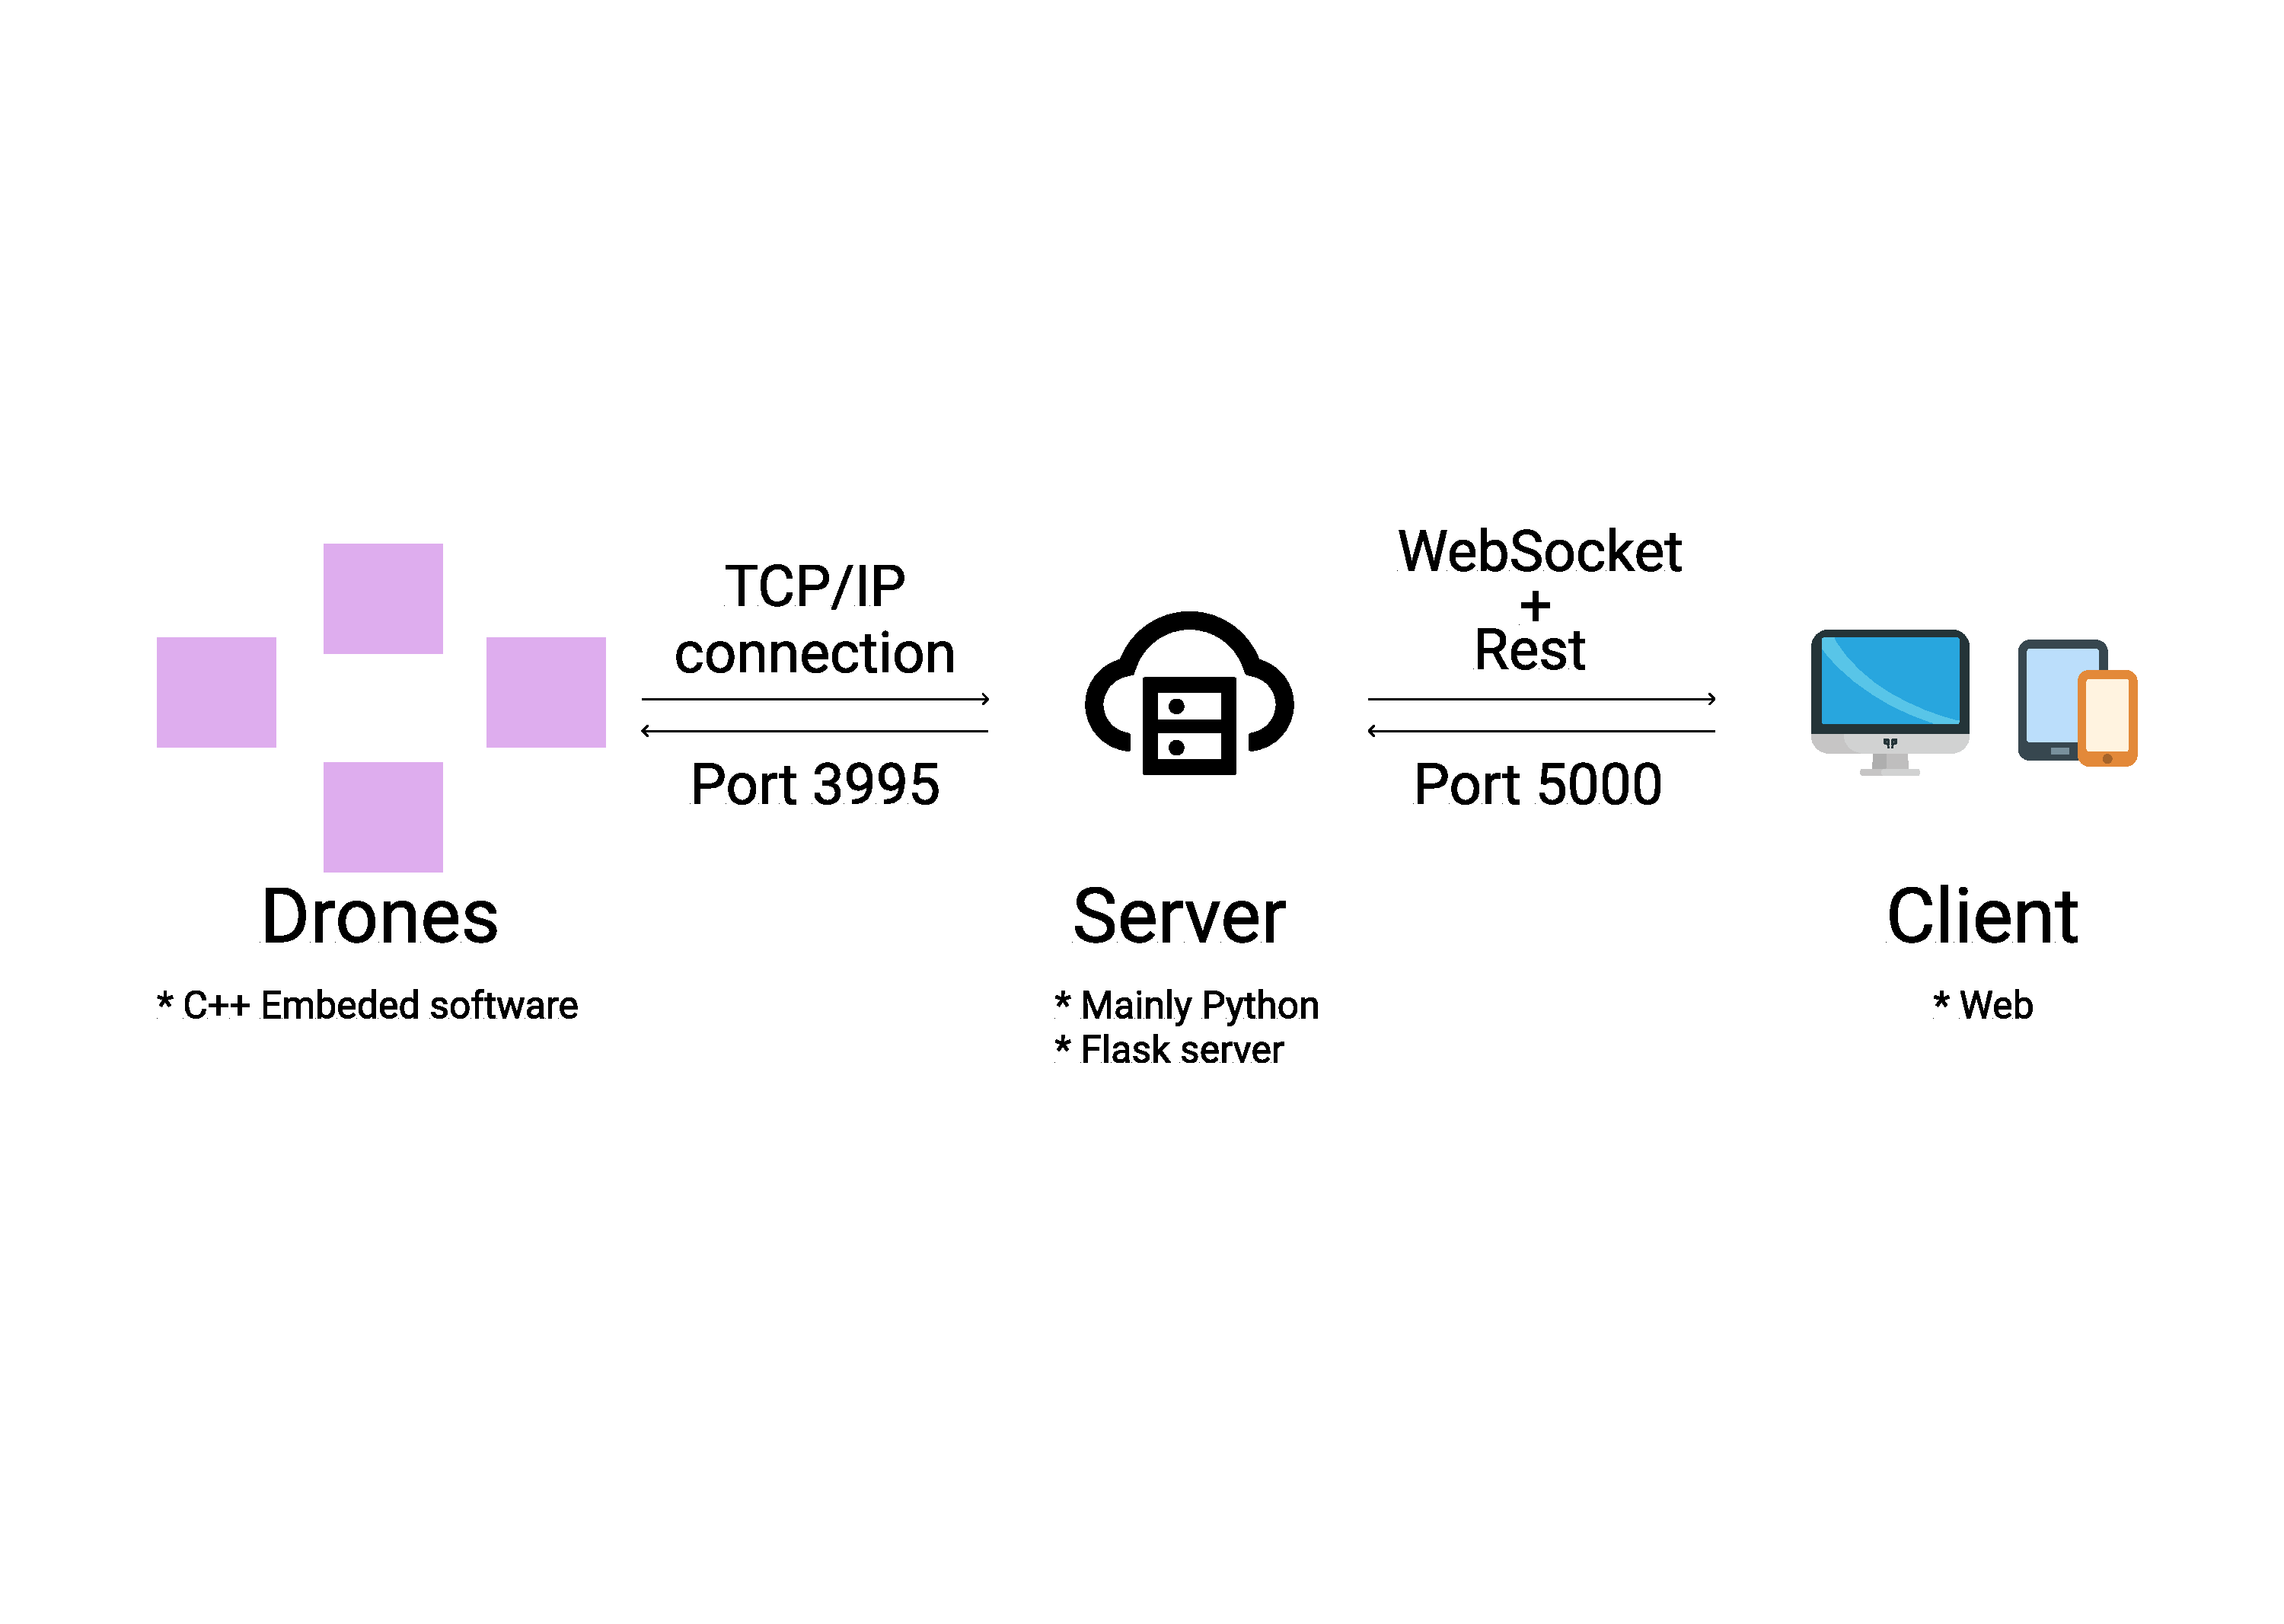
\includegraphics[width=0.9\textwidth]{architecture-globale.pdf}
  \caption{Architecture globale de la solution}
\end{figure}

\par La solution que nous avons retenue fais état de 3 entités :
\begin{itemize}
    \item Un client web : Il s'agit d'une application web utilisé par un opérateur. Il permet ainsi les interactions avec le logiciel des drones
    \item Un serveur maître : Il s'agit d'un serveur centrale qui joue le role d'intermédiaire entre le client et les drones. D'une part il transmettra les commandes du client aux drones. D'autre part, il remettra au client les résultats et informations venant des differents drones.
    \item Les drones : Un ou plusieurs drones qui communiquent entre eux mais également avec le serveur centrale (couple client-serveur). Ils effectuent les activités d'explorations.
\end{itemize}

\par Les requis nous demandent deux modules, à savoir, une station au sol qui est un ordinateur disposant d'une interface web et d'une partie embarqué pour les drones. Nous avons par la suite subdivisé la station au sol en deux éléments qui sont le client et le serveur.

\subsection{Architecture logicielle embarqué}

\textit{Un diagramme qui résume l’architecture.  Un texte qui décrit et justifie les choix.}


\subsection{Architecture logicielle station au sol}

\textit{Quelques blocs des principaux modules ou classes seulement.  Des diagrammes sont nécessaires.  Un texte qui décrit et justifie les choix.}
  

\section{Processus de gestion}

\subsection{Estimations des coûts du projet}

\textit{Les divers frais rattachés au projet peuvent nous aider à estimer le coût global du projet.}
La principale dépense n’est nul autre que les ressources humaines. 
Avec quatre développeur-analyste et un coordonnateur de projet à temps partiel, 
il est nécessaire d’avoir une estimation de temps pour en déduire le coût juste. 
Pour le bien de la cause, nous estimons 11 heures de travail par développeur et 12 heures pour le coordonnateur. 
Sachant que le projet s’échelonne sur 11 semaines, nous obtenons un total de 484 heures pour les développeurs 
et 132 heures pour le coordonnateur. 
En considérant un salaire respectif avoisinant 130\$/h et 145\$/h, le coût humain s’élève à priori à 82060\$. 
Nous disposons de deux drones équipés pour un total 800\$. 
On alloue un 400\$ additionnel qui couvre un possible bris de matériel. 
Le seul logiciel nécessaire est Argos3 et celui-ci ne nécessite aucune license d’utilisation.
L’estimation à priori s’élève donc à 83260\$.

\subsection{Planification des tâches}

\subsubsection{\emph{Preliminary Design Review}}

\begin{center}
  \begin{tabular}{ c c c }
    Date de remise & 15 février 2021 & Samba Bal \\
    
    Serveur WebSocket en Python & 2 heures & Hubert Grootenboer \\
    Construction de l’interface utilisateur avec Angular & 4 heures & Eya-Tom A. Sangam \\
    Client WebSocket dans le fureteur & 3 heures & Eya-Tom A. Sangam \\
    Serveur TCP en Python & 3 heures & Hubert Grootenboer \\
    Client TCP en C++ pour les drones & 3 heures & Issam E. Maghni \\
    Interprétation des commandes de décollage et d’atterrissage dans Argos3 & 2 heure & Mathurin Chritin \\
    Ajout de containers Docker pour les trois modules & 4 heures & Samba Bal
  \end{tabular}
\end{center}

\subsubsection{\emph{Critical Design Review}}

\begin{center}
  \begin{tabular}{ c c c }
    Date de remise & IDK 2021 & Samba Bal \\
    
    Génération aléatoire de l’environnement sur Argos3 & 3 heures & Mathurin Chritin \\
    Ajout de « Return to base » dans l’interface client & 1 heure & Augustin Sangam \\
    Lecture des capteurs et envoie de données & 3 heures & ?? \\
    Communication inter-drones sur ARGoS & 4 heures & Issam E. Maghni \\
    Visualisation de la carte généré à partir de données brutes & 3 heures & IDK \\
  \end{tabular}
\end{center}

\subsubsection{\emph{Readiness Review}}

\begin{center}
  \begin{tabular}{ c c c }
    Date de remise & IDK 2021 & Samba Bal \\
    
    Documentation l’architecture et l’utilisation du système global & 6 heures & IDK \\
    Enregistrement du vidéo décrivant le fonctionnement de la simulation & 2 heures & IDK \\
    Enregistrement du vidéo décrivant le fonctionnement du système sur drone & 2 heures & IDK \\
    Création d’un script permettant de lancer une simulation sur GNU+Linux & 3 heures & IDK \\
    Monter la vidéo 
  \end{tabular}
\end{center}

\subsection{Calendrier de projet}

\textit{Insérer un tableau qui indique les dates cibles de terminaison des phases importantes, des dates de version et autres jalons.  Un résumé seulement.}

\subsection{Ressources humaines du projet}

\textit{Indiquer le nombre et le type de ressources humaines nécessaires, incluant les qualifications spéciales ou l’expérience des membres de l’équipe.}

\par Dans le but de réaliser ce projet nous avons mobilisé 5 ressources. 
 Nous avons un spécialiste du développement d'interface client web principalement Angular. Ce dernier travaille de pair avec un développeur Backend expérimenté. 
 L'équipe dispose de deux développeurs de systême embarqué en C++ avec une expérience non négligeable avec les drones. 

\section{Suivi de projet et contrôle}

Compte tenu des 3 séances hebdomadaires programmées par l'agence spatiale de Polytechnique pour nous rencontrer, des rencontres entre 3 à 5 fois par semaine entre tous les membres de l'équipe sont prévues pour rendre compte de l'avancement de la solution. Des revues de code sont également programmées deux fois par mois, durant lesquelles un des membres de l'équipe devra sélectionner un fichier de code source et le soumettre aux autres membres pour qu'ils l'inspecte et en fassent ensemble une critique constructive. Cela bénéficiera tout autant à la qualité du code final qu'à la cohésion entre les membres de l'équipe.

\subsection{Contrôle de la qualité}

\textit{Tous les biens livrables doivent être soumis à un processus de révision. Une révision est requise afin de s’assurer, au moyen de lignes directrices et de listes de vérification, de la qualité de chaque bien livrable.}
\subsubsection{PDR}
  \begin{itemize}
    \item Le simulateur est fonctionnel et se lance correctement : en appuyant sur play, les deux drones sont à l'arrêt, posés au sol et émettent des « pulse » vers le serveur maître
    \item Une fois le serveur maître lancé, il ne requiert plus aucune intervention humaine
    \item L'interface web est fonctionnelle et ergonomique. Elle présente bien le statut des deux drones en vol dans le simulateur et permet à l'opérateur de cliquer sur un bouton faisant décoller le drone, et sur un autre bouton permettant de le faire atterrir.
    \item Le bouton « TakeOff » a pour effet de faire décoller le drone dans le simulateur
    \item Le bouton « Land » a pour effet de faire atterrir le drone dans le simulateur
    \item Lorsque le drone est en vol, ses informations sont actualisées en temps réel dans l'interface web : niveau de batterie en pourcentage, position \texttt{x, y et z} et vitesse [km/h]
    \item Il est possible de faire voler plusieurs drones à la fois et de les contrôler ensemble depuis l'interface web
    \item Lorsqu'on relance plusieurs fois le simulateur, les drones de l'interface web sont actualisés en conséquence (les drones qui ne sont plus utilisés sont retirés, et les nouveaux drones de la nouvelle instance du simulateur sont ajoutés à leur place)
  \end{itemize}

\subsubsection{CDR}
\begin{itemize}
  \item item1
\end{itemize}

\subsubsection{RR}
\begin{itemize}
  \item item1
\end{itemize}

\subsection{Gestion de risque}

\textit{Par exemple: Lister les principaux risques de ce projet et estimer leur importance.  Donner quelques solutions de remplacement possibles et la façon dont l’équipe entend gérer les changements en cours de projet.}

Le présent document présente un plan organisé des délais et timings à respecter pour le bon déroulement du projet. Le principal risque que nous avons identifié est le non respect de ce planning. Il s'agit ici d'un risque à plusieurs échelles : le non respect d'une tâche assignée une semaine donnée peut être reportée à la semaine suivante sans grandes conséquences. Si ce report déclenche une réaction en chaîne, nous pourrions risquer de ne pas terminer le projet en temps et en heure, ce qui s'avérerait fatal pour le projet d'exploration sur Mars, impliquant des pertes d'argent conséquentes.

Il est donc important pour nous de bien respecter le planning. Pour cela 2 solutions s'offrent à nous : augmenter le nombre d'heure que nous passons sur l'artéfact qui pose problème, ou (dans un cas plus urgent) rayer un certain nombre de fonctionnalités non essentielles prévues dans notre planning.

Un second risque, moins probable, serait que l'un des membres de l'équipe se blesse lors d'une manipulation avec un drone et ne puisse de ce fait plus continuer à travailler sur le projet. Conformément aux consignes de sécurité fournies avec les drones, nous nous devons donc de porter en tout temps une paire de lunettes protectrice pour éviter tout problème qui pourrait nous pénaliser par la suite.

\subsection{Tests}

\textit{Identifier et préciser quelques tests pour chaque sous-système, tant pour le matériel que le logiciel.  Il devrait y avoir un lien entre ces tests et les tâches décrites plus haut.}

\subsection{Gestion de configuration}

\textit{Par exemple : Donner quelques renseignements sur le système de contrôle de version, l’organisation du code source, des tests et les fichiers de données ainsi que la documentation relative au code source et à la documentation de conception.  La séparation et l’intégration entre les fichiers de description du logiciel}

Le code source de la solution sera organisé dans un dépôt GitLab, comprenant 3 sous-\textit{repos} :
\begin{ítemize}
  \item \texttt{drone}, comprenant tout le code C\texttt{++} du micrologiciel embarqué ainsi que les fichiers de configuration du simulateur
  \item \texttt{server}, comprenant tout le code Python du serveur maître qui s'occupera d'interfacer les drones, la base de donnée et l'interface web et d'effectuer un traitement sur les données reçues
  \item \texttt{dashboard}, comprenant l'application Angular qui s'occupera de fournir une interface web à l'opérateur pour le contrôle et l'affichage des données des drones
\end{ítemize}

La documentation du code sera faite avec Doxygen, en générant ainsi 3 PDFs, un par projet, et sera stocké dans les entrepôts associés. Quant à la documentation de la conception, ainsi que la documentation de la solution en générale, elles se trouveront toutes les deux à la racine du dépôt GitLab principal.

\section*{Conclusion}

Bla bla bla

\textbf{Références} avec \texttt{printbibliography.}


\section*{ANNEXES}

\textit{Inclure toute documentation supplémentaire utilisable par le lecteur. Ajouter ou référencer toute norme technique de projet ou plans applicables au projet.}



\end{document}

%%% Local Variables:
%%% mode: latex
%%% TeX-master: t
%%% End:
